\section{Komponenten Optimierer Prototypen}




\begin{figure}[ht]
  \centering
  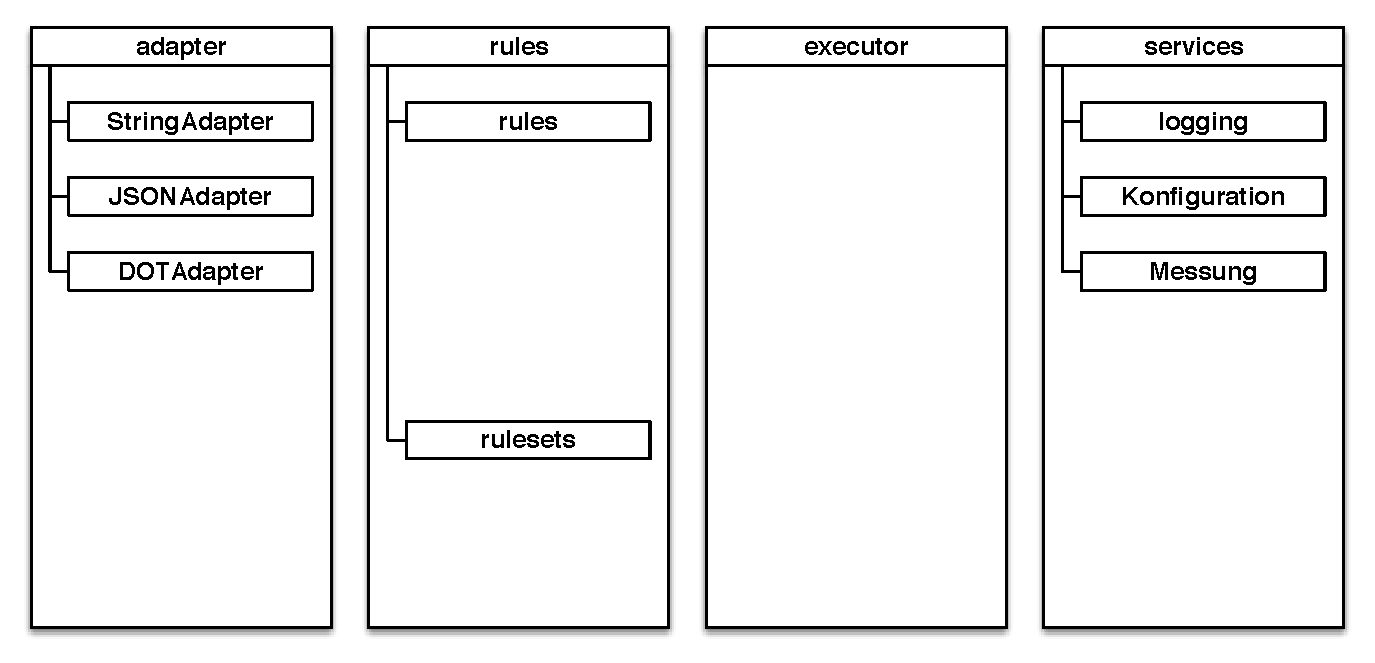
\includegraphics[width=\textwidth]{04_Implementierung/00_media/Organization.pdf}
  \caption{Projektorganisation}
  \label{ProjectOrga}
\end{figure}


Das Projekt ist entlang der unterschiedlichen Aufgaben modular organisiert. Unter dem Dach der Anwendung finden sich vier unterschiedliche Sparten, die gemeinsam für das Ausführen des Programms verantwortlich sind: Planknoten und Äuqivalenzklassen, Regeln und Regelmengen, Ineratoren und Services. Die genaue Zuordnung zu den jeweiligen Bereichen ist in Abb. \ref{ProjectOrga} nachvollziehbar.




Bei der Ausführung eines Tests  müssen alle Bereiche zusammenarbeiten. Der Service-Bereich und insbesondere das Konfigurationsmodul sind für die konkrete Zusammenstellung der für den Test notwendigen Komponenten verantwortlich. Er entscheidet, welche Regeln zum Einsatz kommen, welcher Enumerator gewählt wird, welche konkreten Pläne getestet und mit Hilfe welcher Adapter die Daten ein-  bzw. ausgegeben werden. Um zu verstehen, welche Möglichkeiten das implementierte System bietet, sind die einzelnen Komponenten im Folgenden im Detail beschrieben.




\subsection{Adapter}

Die Implementierung bietet mehrere Adapter, die zur Umwandlung von externen Formaten in eine interne Repräsentationsform, oder von einer internen Repräsentationsform in ein externes Format genutzt werden können. Sie bieten die Möglichkeit andere Systeme an das bestehende System anzudocken und sorgen so für den notwendigen Anschluss und die Erweiterbarkeit durch Dritte.

Insgesamt werden drei Adapter mitgeliefert. (1) JSON\-Adapter, (2) String\-Adapter, (3) DOT\-Adapter.

Der Json-Adapter erlaubt es Daten im JSON Format zu importieren und wird beim Einlesen des initalen Plans genutzt. Er wandelt auf der Basis des Konfigurationsfiles JSON in Planknoten und Äquivalenzklassen um, die dann weiterverarbeitet werden können. Ebenfalls ist es möglich, Pläne in JSON auszugeben. Zu diesem Zweck implementiert der Parser auch eine \texttt{dump} Methode.

Neben dem JSON\-Adapter wird auch ein String Adapter verwendet. Er ist für die Ausgabe von Plänen als String verantwortlich. Im Gegensatz zu einem JSON\-Adapter ist die Eingabe von Plänen mit Hilfe dieses Moduls nicht möglich. Auch der DOT\-Adapter erlaubt nur die Ausgabe von Plänen im DOT\-Format, die  zur Generierung von graphischen Ausgaben verwendet werden können.

Eine weitere Aufgabe eines solchen Adapters kann auch die Übersetzung von Relationsnamen in Bitvektoren sein. Da das vorliegende System, wie in \ref{sec:Bitvector} beschrieben, Relationen als Bitvektoren abbildet, mag es nützlich sein, Relationsnamen in Bitvektoren zu übersetzen. Für diese Übersetzung sind auch Adapter vorgesehen, die zusätzlich implementiert werden können.












\subsubsection{Erweiterbarkeit von Regelsets}





\subsubsection{Ausführung von Regeln}

Das eigentliche Ausführen der Regeln wird durch einen XY durchgeführt. Im konkreten Fall kommt hier der Algorithmus ExhaustiveTransformation zum Einsatz. Der Algorithmus startet mit einer Äquivalenzklasse. Innerhalb dieser Äquivalenzklasse werden die Regeln, die durch ein Regelset vorgegeben sind auf einem PlanKnoten ausgeführt. Die Ausführung geschieht hierbei zuerst auf den Oberen Ebenen und setzt sich dann auf den Kindern eines Knoten fort. Somit können bei der Transformation eines gegebenen Baums alle Regeln auf andere Bäume angewendet werden.

Wichtig ist hierbei zu bemerken, dass dieser Algorithmus immer zuerst prüft, ob eine Regel auch tatsächlich für die Anwendung geeignet ist und dann erst der Algorithmus ausgeführt wird. Neben der eigentlichen Eignung wird auch geprüft, ob eine Äquivalenzklasse bereits vollständig expandiert wurde. Falls dies der Fall ist, wird von einer weiteren Anwendung von Regeln abgesehen. Diese Funktion kann insbesondere Vorteile bei der Implementierung von neuen Regelsets bieten. Nutzt ein gegebenes Regelset die Möglichkeit nicht nur einen neuen Planknoten zu generieren, sondern gleich mehrere Planknoten zu erstellen und auch in diesem Zusammenhang bereits mehrere Kinder-Knoten zu erstellen, kann die Reihenfolge der Expansion von Äuqivalenzklassen geändert werden. Die einzelnen Äquivalenzklassen, die bereits durch eine Regel expandiert wurden, werden als solche markiert und die bisher vorhandenen Regeln werden nicht mehr ausgeführt.















